\chapter{Přenos momentu síly}

Možnost vytváření takto magneticky vázaných spinnerů je slibnou známkou toho, že bude opravdu možné využít takovýto systém jako funkční převod. Kromě poměru otáček na vstupu a výstupu je ale k vytvoření použitelného převodu potřeba určit i moment síly, který je taková převodovka schopna přenášet.

\section{Úprava aparatury}

K tomu, abychom změřili přenesený moment síly, lehce upravíme naši předchozí aparaturu popsanou v kapitole \ref{sub:main_2LS_aparature}. Tato úprava spočívá v připevnění pevného, ale lehkého, plechového obdélníku k hnanému spinneru, který bude působit jako zátěž. Moment síly, kterým plech působí na spinner, vychází z odporu vzduchu, kterému je plech podroben. Výhodou tohoto řešení je, že zátěž dynamicky roste s otáčkami, což nám později umožní jednoduše hledat maximální přenositelný moment v závislosti na několika relevantních parametrech této rudimentární převodovky. Alternativní řešení, jako například vytváření umělého tření na spinneru, kde by přenášený moment byl počítán ze smykového tření dvou styčných ploch o známých vlastnostech, má značné nevýhody jako například: 

\begin{enumerate}[topsep=0pt, partopsep=0pt]
    \setlength{\itemsep}{0pt}%
    \setlength{\parskip}{0pt}%
    \item \textbf{Nedynamičnost v závislosti na rychlosti} - Idealizované smykové tření se narozdíl od odporu vzduchu nemění s rychlostí, což znamená, že by bylo potřeba vytvořit specifickou aparaturu pro každý přenášený moment, který bychom si přáli změřit.
    \item \textbf{Konstrukční náročnost} - Vytváření mnohých styčných ploch různých velikostí a potřeba je udržet perfektně v kontaktu na tak malém objektu jako je fidget spinner je nesrovnatelně konstrukčně složitější, než námi nabízené řešení.
\end{enumerate}

Když nám byl jasný způsob vytváření zátěže, stačilo už jen jeden ze spinnerů permanentně upravit přidáním tohoto plechu. Čepel tohoto jednoduchého "větráčku" byla připojena pomocí pevného drátu, lepící pásky a lepidla k tělu spinneru tak, aby drát nijak nezasahoval do ložiska a neměnil vlastnosti spinneru samotného. Strategickým ohnutím drátu jsme pak byli schopni čepel umístit jejím středem co nejblíže k ose otáčení spinneru. Bohužel, toto nebylo perfektní, a tak budeme muset později provádět lehkou korekci v jednom z našich výpočtů.
Výsledný vzhled upraveného spinneru je na obrázku \ref{fig:dragfoil_spinner}.

\clearpage

\section{Popis chování}

\begin{wrapfigure}{r}{0.45\textwidth}
    \vspace{-1cm}
    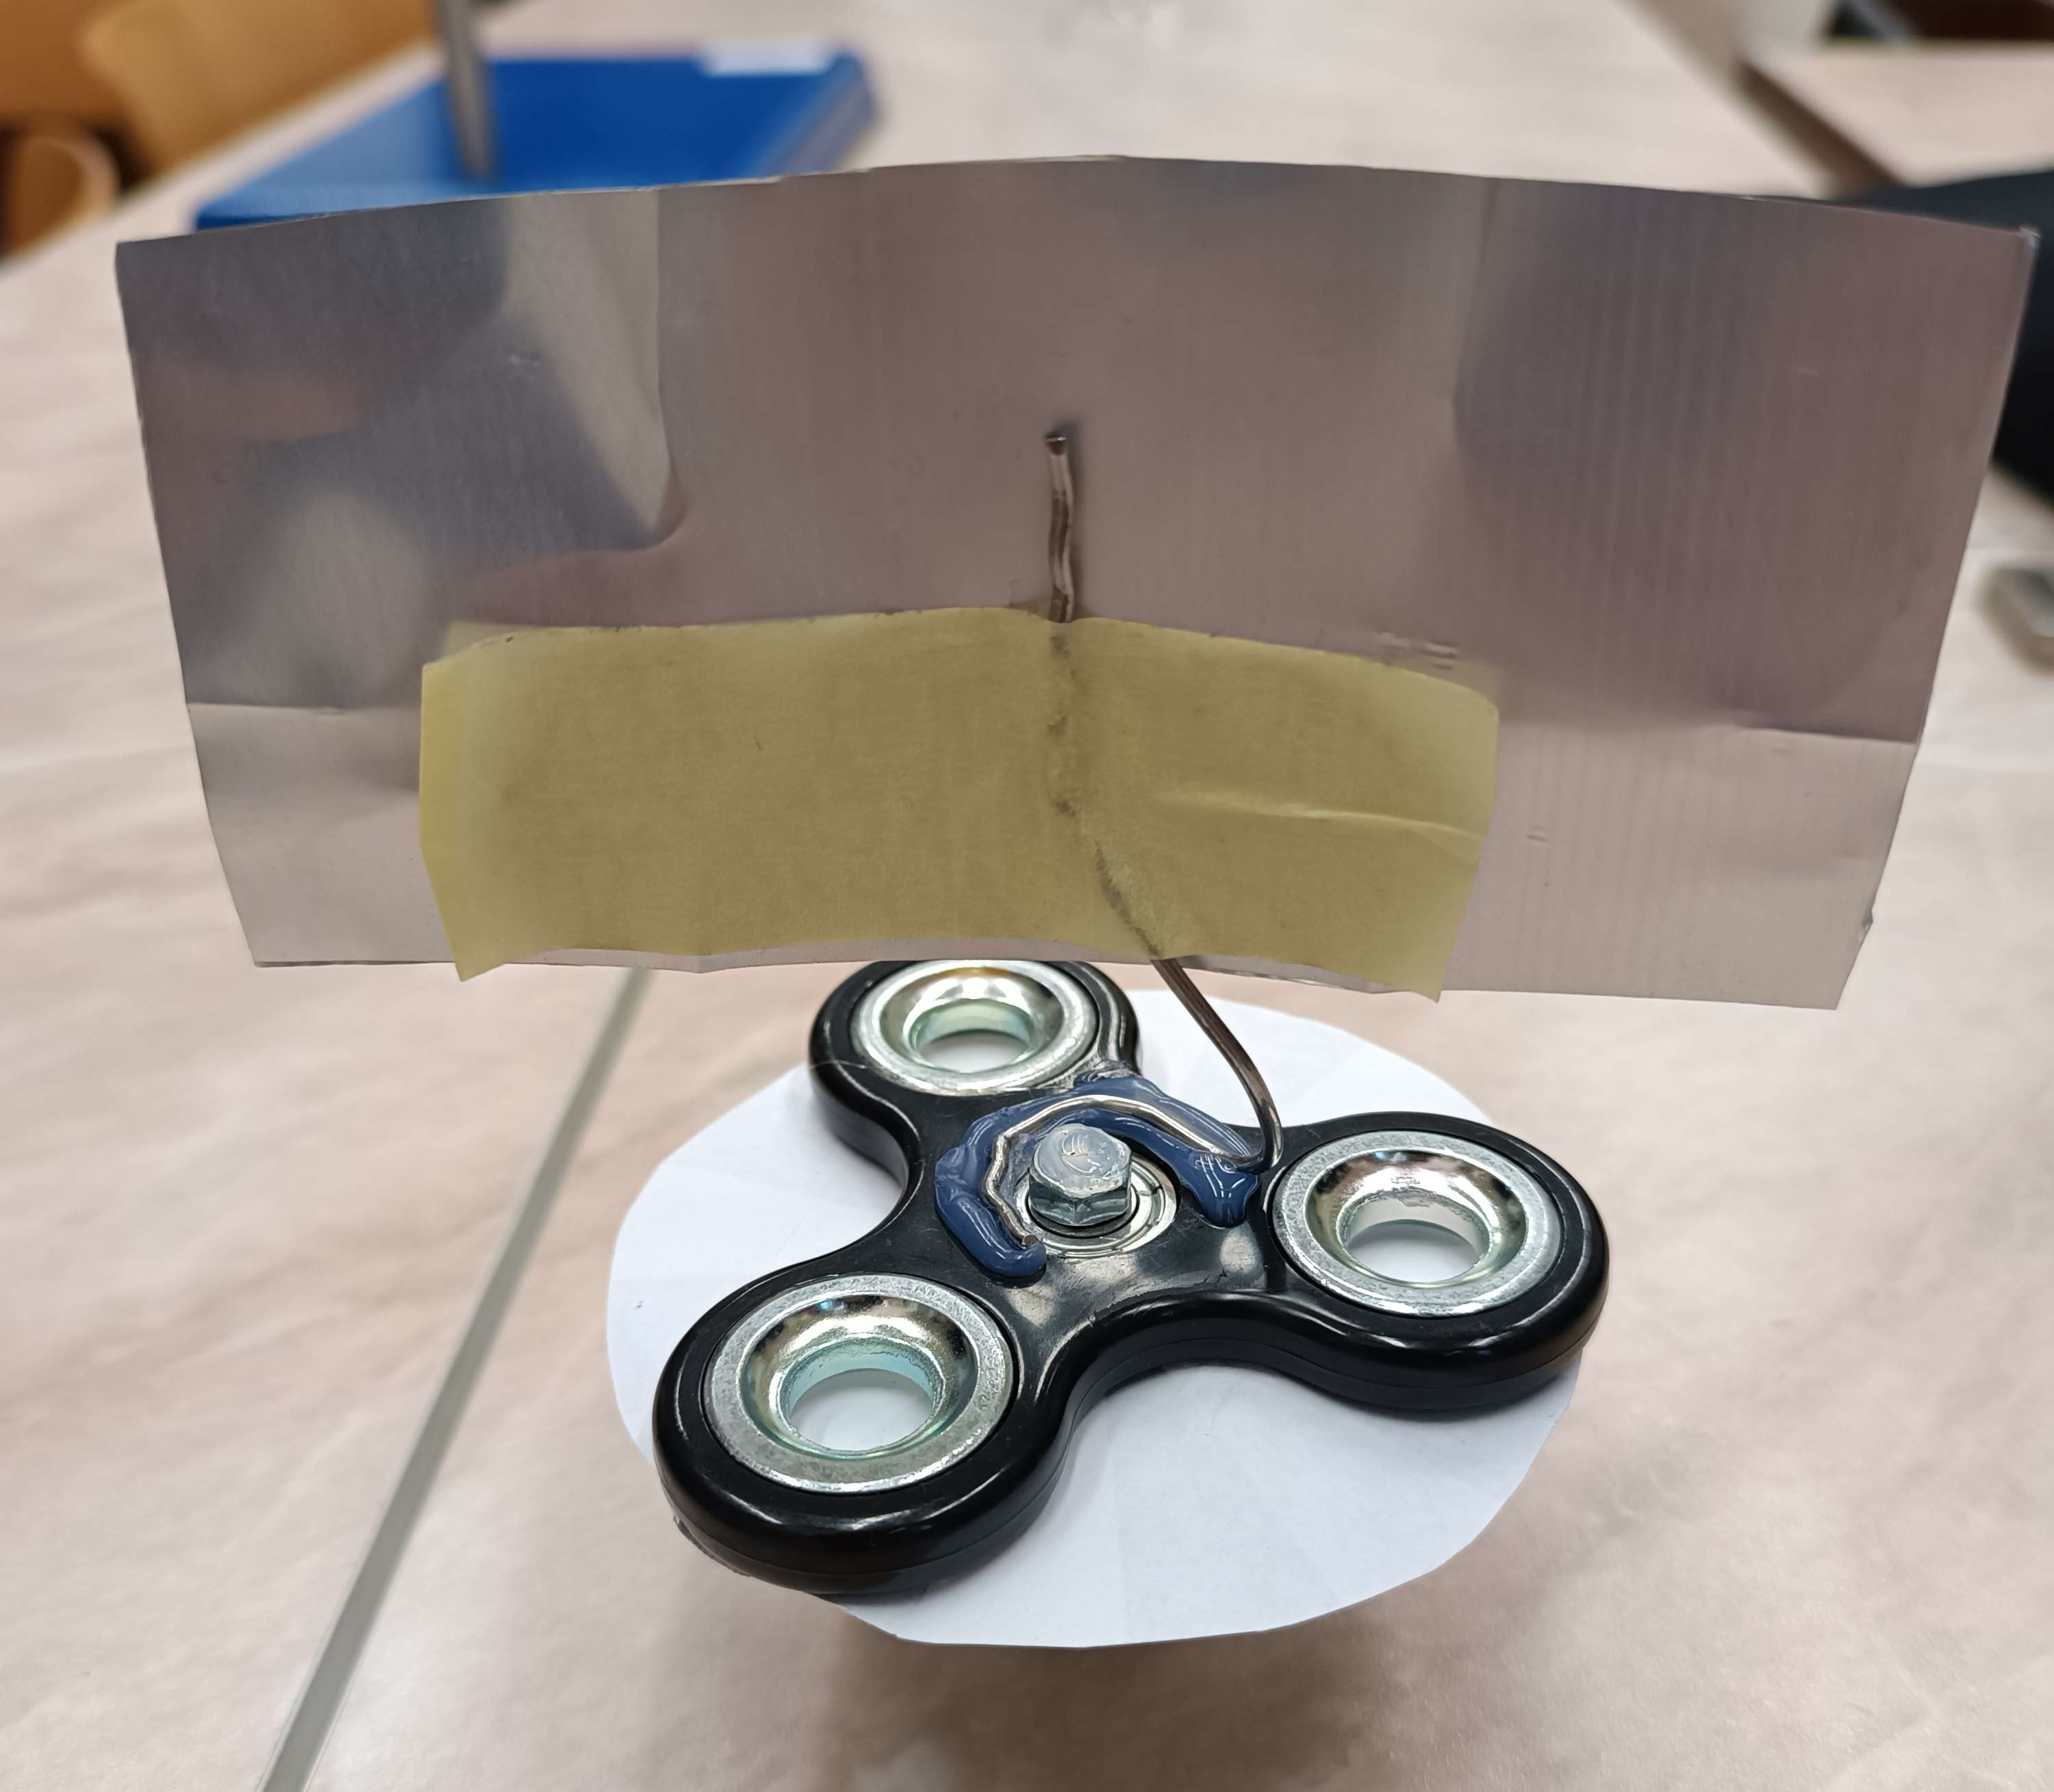
\includegraphics[width=0.45\textwidth]{dragfoil_spinner.png}
    \centering
    \caption{Spinner upravený k měření přenášeného momentu síly.}
    \label{fig:dragfoil_spinner}

    \vspace{1cm}
    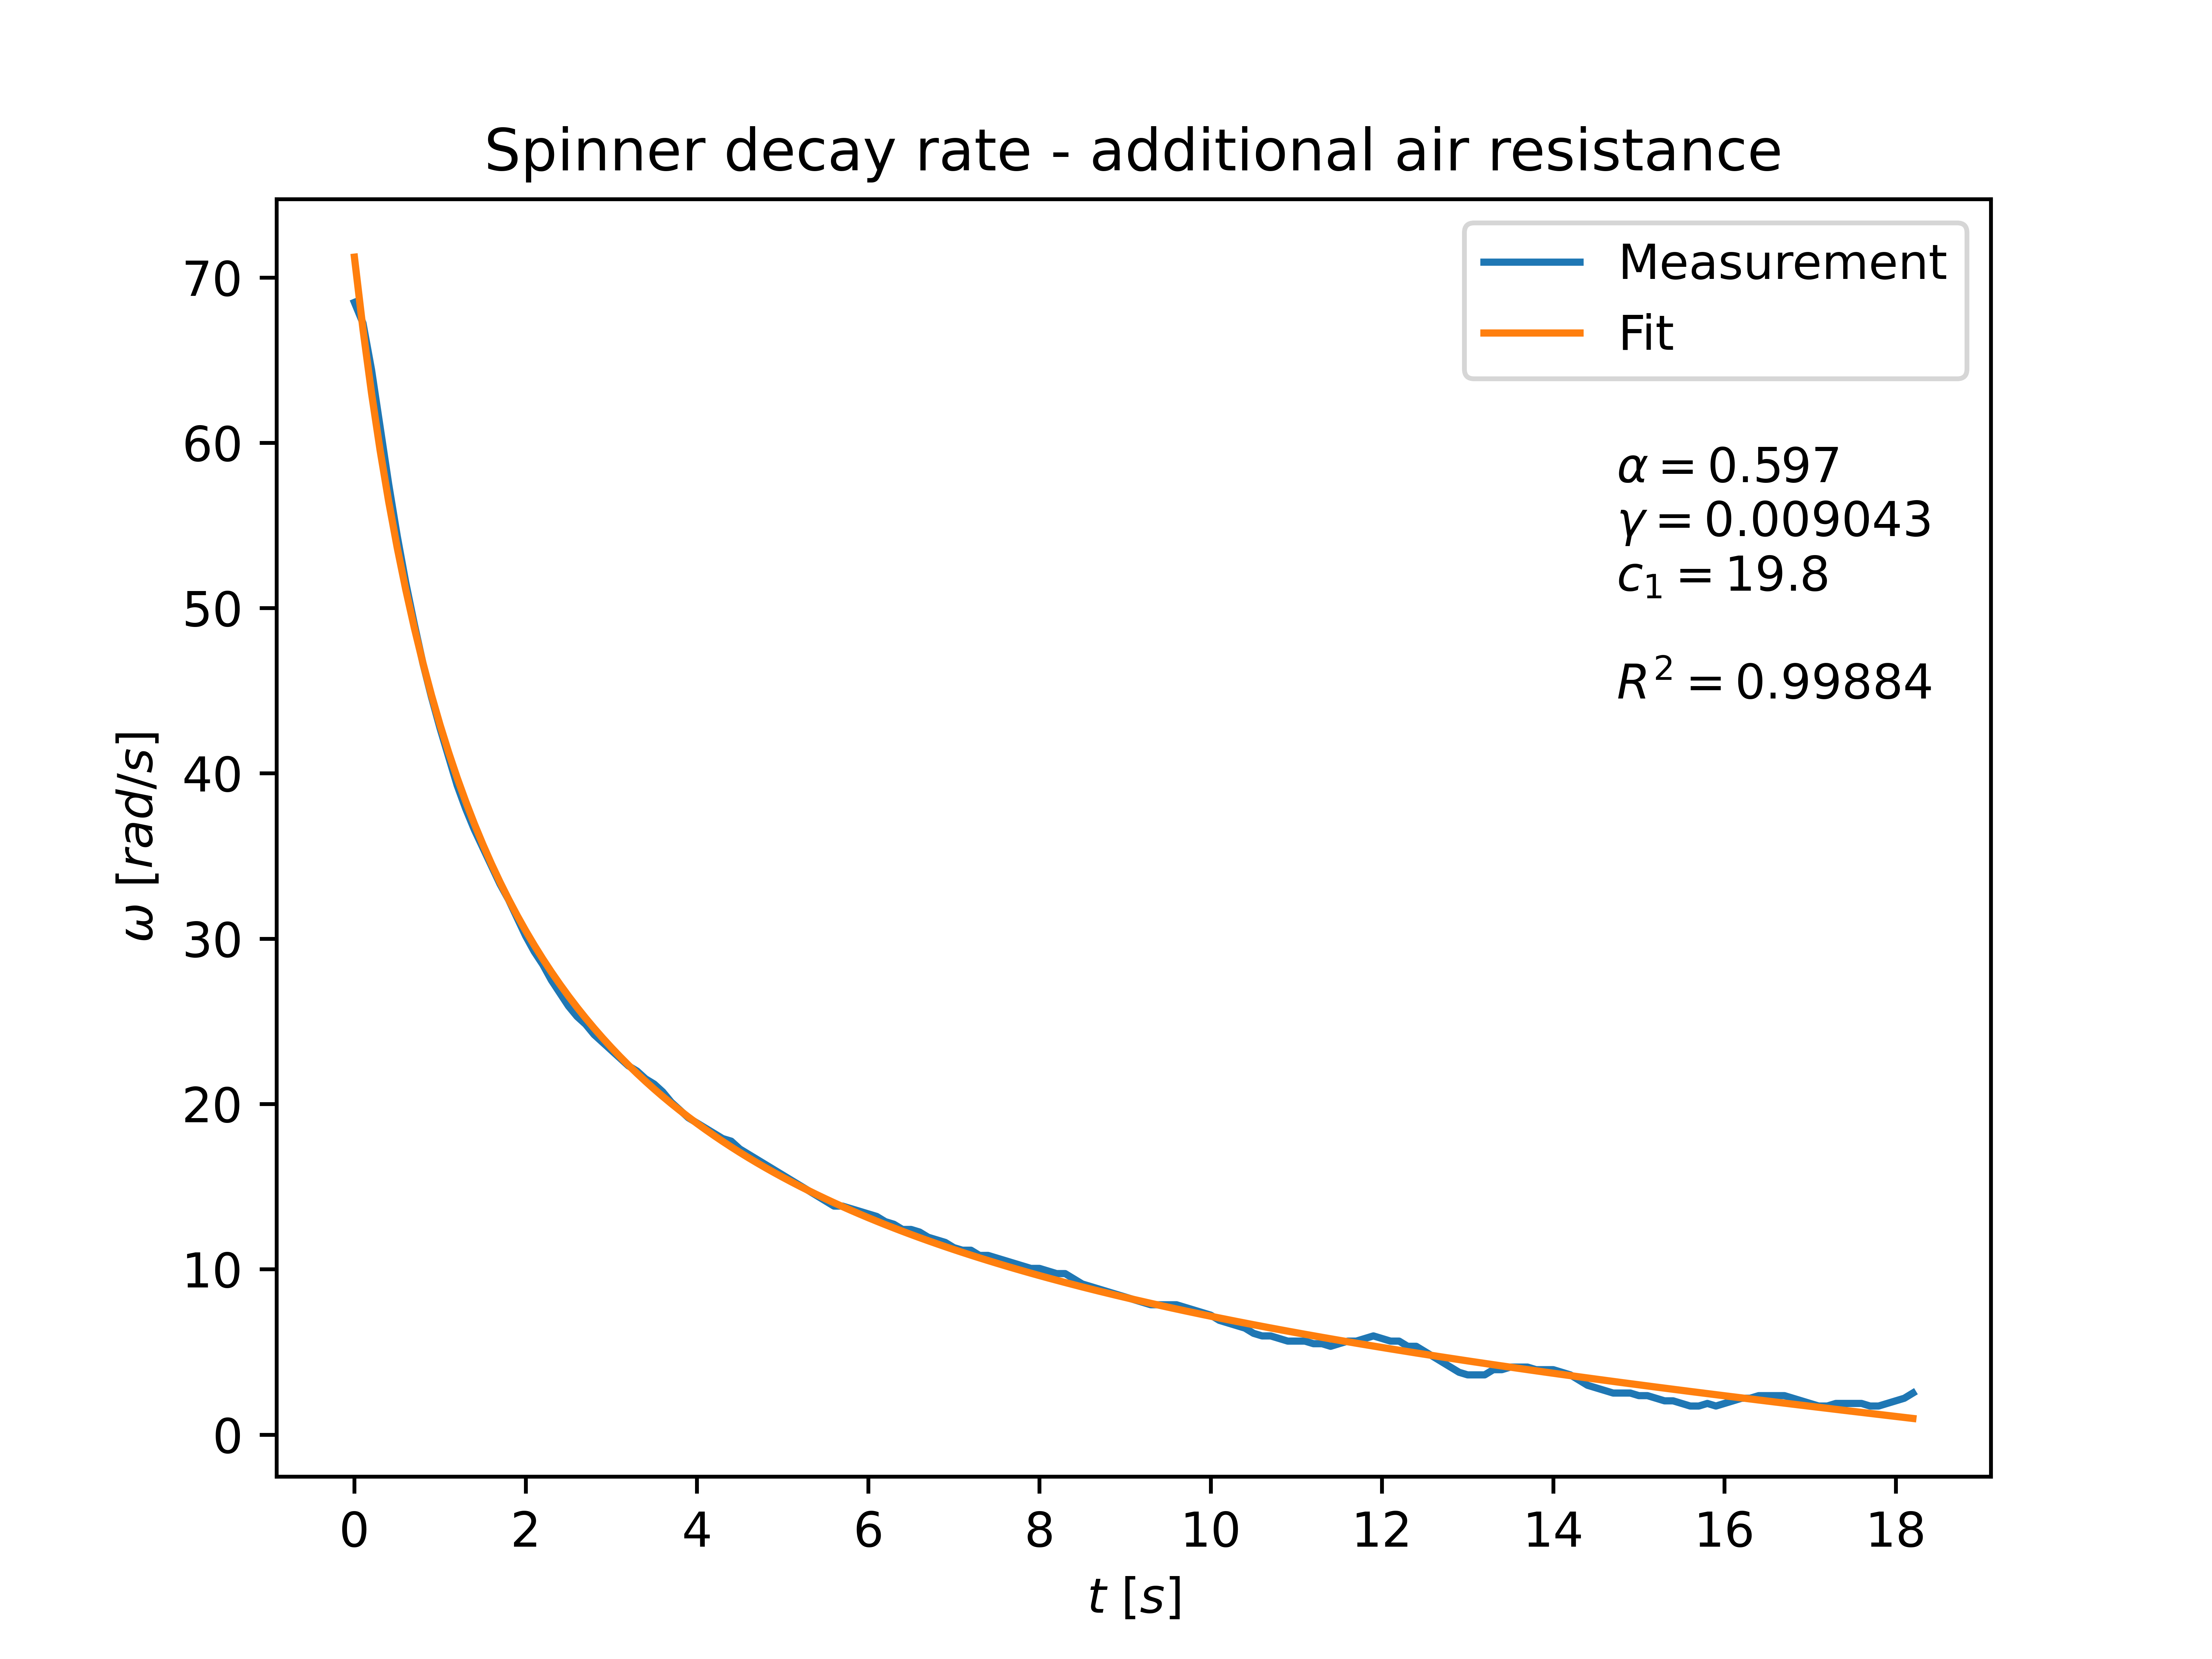
\includegraphics[width=0.45\textwidth]{dragfoil_spinner_decay.png}
    \centering
    \caption{Výsledky měření k určení třecích koeficientů spinneru.}
    \label{fig:dragfoil_spinner_decay}
\end{wrapfigure}

V předchozích experimentech jsme tření vycházející z odporu vzduchu popisovali naším třecím koeficientem $\gamma$. Nyní jsme čistě pro kontrolu toho, že námi udělané změny opravdu měly dopad hlavně na odpor vzduchu, provedli měření, kdy jsme spinner roztočili  náhodou rychlostí a nechali ho pomalu zpomalit pouze vlastním třením. Poté jsme k analýze těchto dat použili náš předchozí algoritmus (viz kód \ref{code:3} a \ref{code:4}) a data jsme fitovali stejně jako v grafech \ref{fig:drag_fit}, \ref{fig:drag_fit_wlin}, \ref{fig:drag_fit_mag}, \ref{fig:drag_fit_mag_wlin}, čímž jsme určili nové koeficienty $\alpha$ a $\gamma$ pro tento upravený spinner. Výsledky této prvotní analýzy jsou k vidění na grafu \ref{fig:dragfoil_spinner_decay}.

Jak je z fitu zřejmé, náš analytický popis tření byl stále úspěšně schopen popsat i tento případ. Naměřený koeficient $\gamma = 9.04\cdot10^{-3} \text{ } rad^{-1}$ v tomto případě vychází přibližně 30 krát větší, než v původních měřeních těchto koeficientů pro holé spinnery (viz \autoref{eq:drag_coef_res}). Koeficient $\alpha$ se udržuje stále v původním rozmezí a naše úpravy na něj tedy měly zanedbatelný dopad.

Když víme, že naše úpravy měly kýžený efekt na chování spinneru, přejdeme k určení závislosti brzdného momentu $\tau_{braking}$ v závislosti na rychlosti otáčení.

{
    \raggedright
    \subsection{Hrubý matematický model}
    Nejdříve se pokusíme o vytvoření hrubého matematického modelu, kterým se pokusíme závislost $\tau_{braking}$ na $\omega$ popsat. K tomuto použijeme klasický středoškolský vzoreček pro výpočet odporové síly turbulentního proudění:
}

\begin{equation}
    \label{eq:highschool_drag}
    \begin{gathered}
        F = -\frac{1}{2} \rho C_D S v^2
    \end{gathered}
\end{equation}

\clearpage

Tento vzorec využijeme k výpočtu síly v každém bodě plechu. Pro každý bod poté vypočítáme vlastní moment síly přes rameno (neboli jeho vzdálenost od osy otáčení) a integrováním přes celou plochu získáme celkový brzdný moment.

Zde také budeme muset zapojit dříve zmíněnou kompenzaci pro to, že střed plechu v našem případě byl posunut přibližně $5mm$ od osy otáčení spinneru. Rozdělíme tedy celou plochu na dvě části - levou (o šířce $R_{left}$) a pravou (o šířce $R_{right}$), kde jedna z nich bude o $5mm$ širší a druhá o $5mm$ užší něž je polovina celé šířky plechu. Výpočet je pak následující:

\begin{equation}
    \label{eq:braking_torque}
    \begin{gathered}
        \tau_{braking} = \int_{-R_{left}}^{R_{right}} \big( F(r) \times r \big) \,dS \\
        \quad \Big\Downarrow \scriptscriptstyle{F(r) \perp r} \vphantom{\Bigg(} \\
        \tau_{braking} = \int_{-R_{left}}^{R_{right}} \Big( -\frac{1}{2} \rho C_D v^2 r \Big) \,dS \\
        \scriptscriptstyle{S = h \cdot r} \Big\Downarrow \scriptscriptstyle{v = \omega \cdot r} \vphantom{\Bigg(} \\
        \tau_{braking} = \int_{-R_{left}}^{R_{right}} \Big( -\frac{1}{2} \rho C_D h (r \omega)^2 r \Big) \,dr \\
        \tau_{braking} = -\frac{1}{2} \rho C_D h \omega^2 \int_{-R_{left}}^{R_{right}} r^3 \,dr \\
        \tau_{braking} = -\frac{1}{8} \rho C_D h \big( R_{right}^4 + R_{left}^4 \big) \omega^2
    \end{gathered}
\end{equation}

Po dosazení tabulkové hodnoty hustoty vzduchu, změřených rozměrů plechu\footnote{Změřené rozměry plechu byly: $h = 5.2cm$, $R_{left} = 5.55cm - 0.5cm$ a $R_{right} = 5.55cm + 0.5cm$} a činitele odporu $C_D$, získáme závislost $\tau_{braking}$ na $\omega$. Činitel odporu se těžko určuje, ale pro tento hrubý odhad jsme vybrali hodnotu 1.4, jelikož plech je zároveň částečně konkávně prohnutý\footnote{Zde vycházíme z hodnot určených v knize \textit{Fluid-Dynamic Drag} od Sigharda F. Hoernera \cite{plate_drag_coef}.}.

K brzdnému momentu pak můžeme ještě připočítat třecí koeficient spinneru, čímž získáme finální hrubý odhad:

\begin{equation}
    \label{eq:braking_torque_w_spinner_drag}
    \begin{gathered}
        \tau_{braking} = -\frac{1}{8} \rho C_D h \big( R_{right}^4 + R_{left}^4 \big) \omega^2 -I\gamma\omega^2
    \end{gathered}
\end{equation}

\clearpage

\subsection{Měřená $\tau-\omega$ závislost}

Vyjádřením $\tau_{braking}$ v závislosti na $\omega$ pomocí třecích koeficientů naměřených v grafu \ref{fig:dragfoil_spinner_decay} získáváme:
\begin{equation}
    \label{eq:braking_torque_from_coefs}
    \begin{gathered}
        \omega(t) = - \sqrt{\frac{\alpha}{\gamma}} \tan{(\sqrt{\alpha\gamma}(t+c_1))} \\
        \tau_{braking} = I\dot{\omega} = -I\alpha \sec^2(\sqrt{\alpha \gamma} (t + c_1))
    \end{gathered}
\end{equation}

Naměřená závislost celkového brzdného momentu na úhlové rychlosti, odpovídající analytický fit, kvadratický fit a konečně hrubý magnetický model (včetně členu $-I\gamma\omega^2$) jsou vyobrazeny v grafu níže:

\begin{figure}[H]
    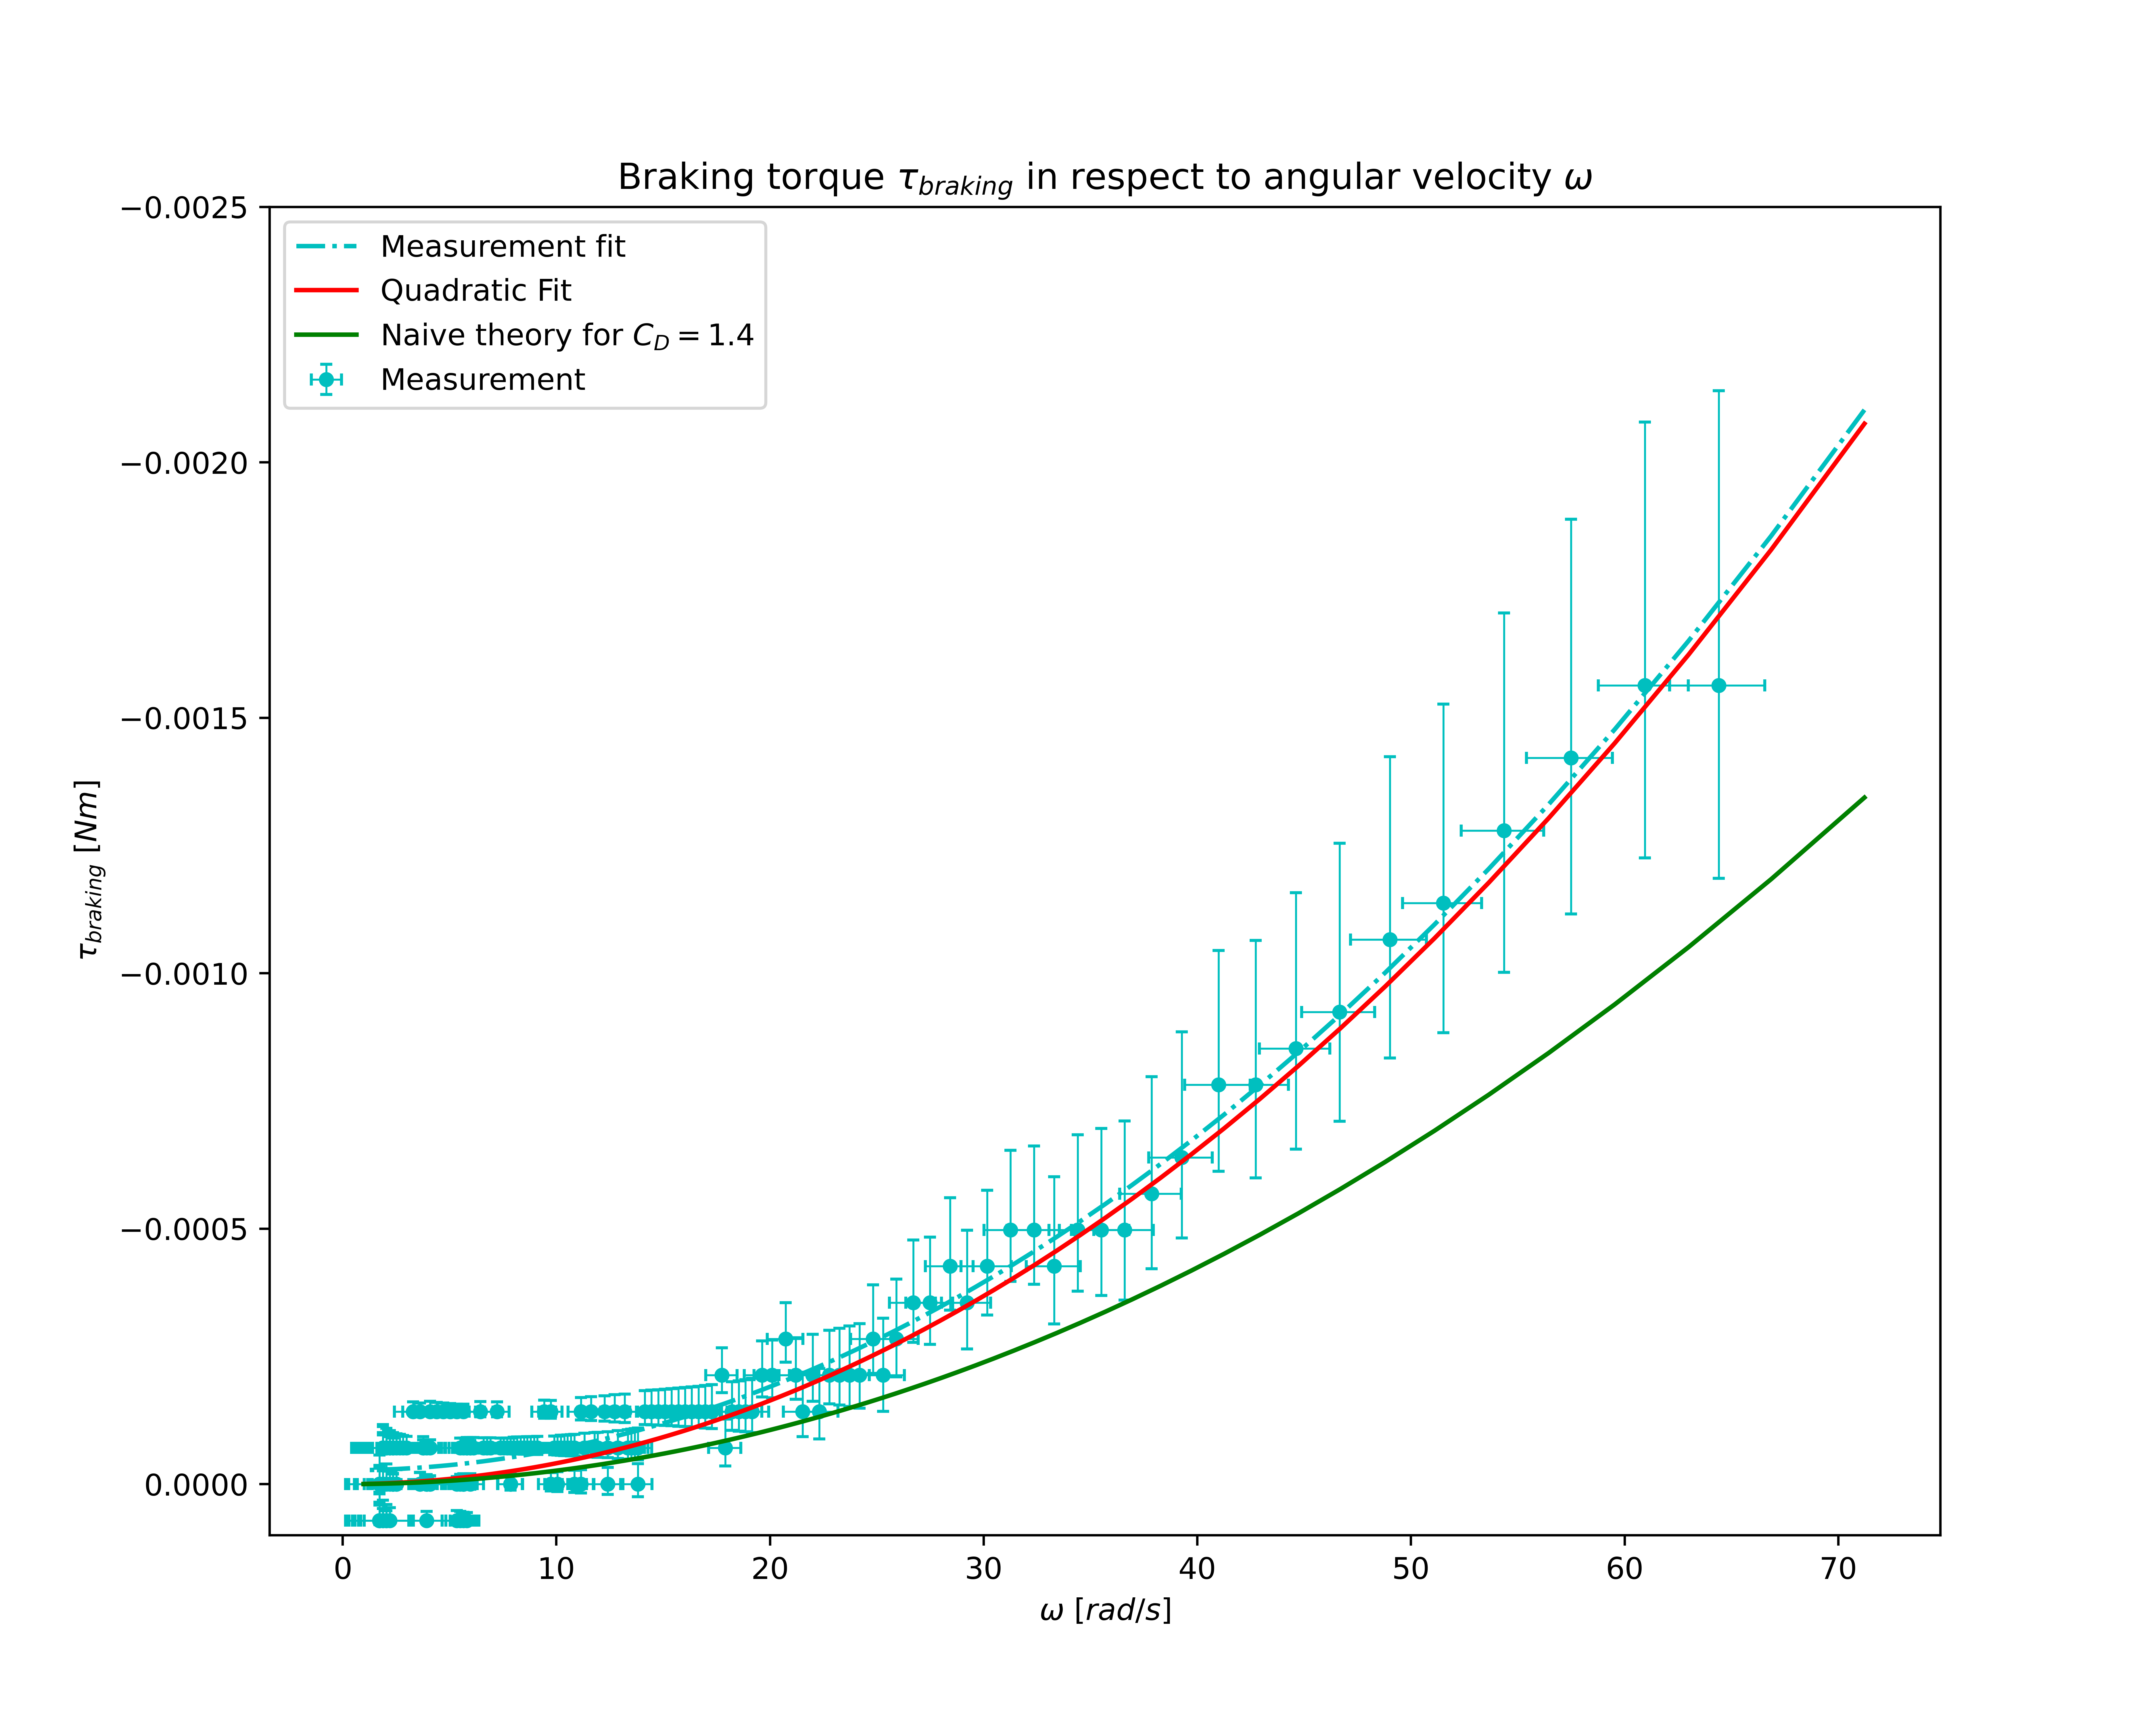
\includegraphics[width=0.85\textwidth]{braking_torque_in_omega.png}
    \centering
    \caption[Závislost brzdného momentu na úhlové rychlosti]{Závislost měřeného brzdného momentu na úhlové rychlosti v porovnání s hrubým modelem}
    \label{fig:braking_torque_in_omega}
\end{figure}

Jak můžeme vidět, čistě kvadratický fit velmi dobře popisuje tuto závislost, což bychom očekávali vzhledem k původní rovnici \ref{eq:highschool_drag}. Dále budeme přenesený moment síly počítat pouze takto: 
\begin{equation}
    \label{eq:torque_transf_final}
    \begin{gathered}
        \tau(\omega) = -4.09\cdot10^{-7}\omega^2
    \end{gathered}
\end{equation}

\clearpage

\section{Měření přenosu}

Pomocí nové aparatury jsme schopni určit maximální přenášený moment síly pro různé konfigurace. Tuto hodnotu zjistíme tak, že budeme hnací spinner pomalu roztáčet rychleji a rychleji (pomocí zvyšování napětí na laboratorním zdroji), dokud se vazba mezi hnacím a hnaným spinnerem se zátěží nerozbije. Z nejvyšší hodnoty napětí zpětně dopočítáme úhlovou rychlost (viz \autoref{fig:motor_characteristic}) a z úhlové rychlosti dopočítáme maximální přenesený moment. Vždy budeme udržovat vazbu v módu 1:1, protože jiné módy jsou moc citlivé a nespolehlivé.

\begin{wrapfigure}{r}{0.5\textwidth}
    \vspace{-1cm}
    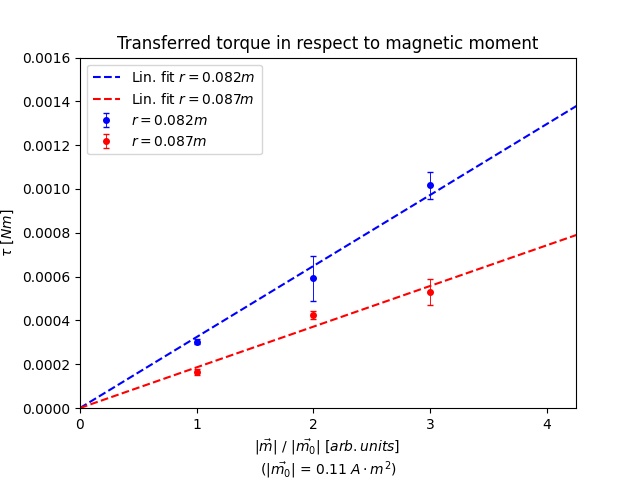
\includegraphics[width=0.5\textwidth]{torque_trans_mag_mom.png}
    \centering
    \caption{Závislost přenášeného momentu na velikost magnetického momentu}
    \label{fig:torque_trans_mag_mom}

    \vspace{1cm}
    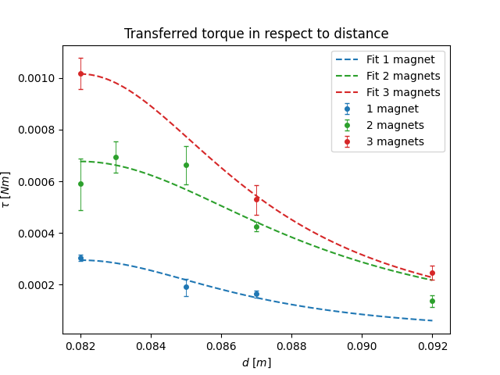
\includegraphics[width=0.5\textwidth]{torque_trans.png}
    \centering
    \caption{Závislost přenášeného momentu na vzdálenosti spinnerů}
    \label{fig:torque_trans}
\end{wrapfigure}

Co se konfigurací týče, budeme sledovat dva hlavní parametry: vzdálenost spinnerů a velikost magnetických momentů (resp. počet magnetů na každém ramenu). Pro každou kombinaci parametrů budeme měření opakovat 2-4 krát. Nejdříve se podíváme na výsledky závislosti momentu na počtu magnetů (viz graf \ref{fig:torque_trans_mag_mom}).

Po zpracování dat vyplyne přibližně lineární závislost mezi přenosem a počtem magnetů. Zároveň tato závislost vychází pouze ze tří bodů a celkem 10 měření, což určitě není dostatečné k vytvoření definitivního závěru. Také byly měřeny pouze případy s poměrně "malým" počtem magnetů, protože více magnetů se nedalo dobře ke spinneru připevnit.

Druhá závislost, závislost na vzdálenosti, vykazuje úměrnost\footnote{Přesnější popis této úměrnosti je $\tau \propto \big( \sqrt{k^2+(d-2r)^2} \big)^{-4}$. $k$ v tomto případě představuje nějakou minimální vzdálenost v tečném směru, kterou si od sebe magnety vždy udržují (např. půl délky sub-periody, pokud by byly spinnery perfektně zaklesnuty). $d$ představuje vzdálenost středů spinnerů. $r$ je poloměr spinneru. } $\tau \propto r^{-4}$, která odpovídá rovnici \ref{eq:F_m}. Velká vzdálenost spinnerů hraje tedy hlavní roli ve velikosti přenášeného momentu.

\clearpage